%%%%%%%%%%%%%%%%%%%%%%%%%%%%%%%%%%%%%%%%%%%%%%%%%%%%%%%%%%%%%%%%%%%%%%%%%%%%%%%%
%2345678901234567890123456789012345678901234567890123456789012345678901234567890
%        1         2         3         4         5         6         7         8
% THESIS CHAPTER

\chapter{First chapter}
\label{chap:first}
\ifpdf
    \graphicspath{{Chapter1/Figures/PNG/}{Chapter1/Figures/PDF/}{Chapter1/Figures/}}
\else
    \graphicspath{{Chapter1/Figures/EPS/}{Chapter1/Figures/}}
\fi

% short summary of the chapter
\section*{Summary}

Examples of commonly used commands.

\section{Basic commands}
\label{sec:basic_commands}

This is a citation: \cite{Cox91}.

This is an emphasized word: \emph{global}.

This is a reference to another part of the thesis: Chapter \ref{chap:introduction}.

This is an enumerated list:
\begin{enumerate}
\item first item.
\item second item.
\end{enumerate}

This is an in-line equation: $x-$.

This is a word in quotes: ``regular''.

\section{Equation}
\label{sec:equation}

This is an equation:
\begin{equation}
{\mathcal{U}}_k(s_k) = \frac{P_k}{C_k}
\label{eq:normal}
\end{equation}

This is an equation split over multiple lines:
\begin{equation}
\begin{array}{l}
x_{k}={\mathcal{F}}(x_{k-1},u_{k},w_{k-1})\\
z_{k}={\mathcal{H}}(x_{k},v_{k})
\label{eq:Split}
\end{array}
\end{equation}

This is one hell of an equation:
\begin{equation}
\begin{array}{c}
 \mathcal{Q}_l  = \frac{{d_l ^2 \sigma _\phi  ^2 }}{2}\left[ {\begin{array}{cc}
   {2\sin ^2 \phi _l } & { - \sin 2\phi _l }  \\
   { - \sin 2\phi _l } & {2\cos ^2 \phi _l }  \\
\end{array}} \right] +
 \begin{array}{cc}
   {\frac{{\sigma _d ^2 }}{2}\left[ {\begin{array}{cc}
   {2\cos ^2 \phi _l } & {\sin 2\phi _l }  \\
   {\sin 2\phi _l } & {2\sin ^2 \phi _l }  \\
\end{array}} \right]}  \\
\end{array} \\
 \end{array}
\label{eq:defQ}
\end{equation}

This is a reference to the Equation \ref{eq:Split}.

\section{Figure}
\label{sec:figure}

%I add a figure.
%\begin{figure}
%\centering
%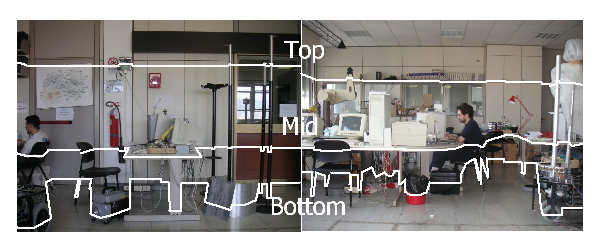
\includegraphics[width=5.0in]{Views}
%\caption{Scan profiles: \emph{bottom}, \emph{mid} and \emph{top view}.}
%\label{fig:views}
%\end{figure}

This is a reference to Figure \ref{fig:views}.

\section{Algorithm} 
\label{sec:algorithm}

This is an algorithm:
\begin{algorithm}
\label{alg:SMS}
\caption{Split \& Merge [\& Split]}
\begin{algorithmic} [1]
\REQUIRE{A scan $s$. A stack $\mathcal{L}$. A counter $j$. A threshold $\tau$}
\ENSURE{$\lambda \leftarrow \mathcal{M}(s)$, $j=1, ..., |\lambda|$}
\STATE{$\mathcal{L}$ = \texttt{push}($s$)}
\STATE{$j \leftarrow 1$}
\WHILE{$\mathcal{L}$ $\neq$ $\varnothing$}
\STATE{$\mathcal{L}$ = \texttt{pop}($s_{top}$)}
\STATE{$l_j$ $\leftarrow$ \texttt{fitting}($s_{top}$)}
\STATE{$q_k = \argmax_{q}\texttt{dist(l$_j$,q)}$}
\IF{$\texttt{dist(l$_j$,$q_k$)} < \tau$}
\STATE{$j \leftarrow j+1$}
\STATE{\texttt{continue}}
\ELSE
\STATE{$s_a \leftarrow$ \texttt{sub}($s_{top}$, 1, $k$)}
\STATE{$s_b \leftarrow$ \texttt{sub}($s_{top}$, $k+1$, $|s|$)}
\STATE{$\mathcal{L}$ = \texttt{push}($s_a$)}
\STATE{$\mathcal{L}$ = \texttt{push}($s_b$)}
\ENDIF
\ENDWHILE
\STATE{\{$l_j$\} $\leftarrow$ \texttt{merge}(\{$l_j$\})}
\STATE{\{$l_j$\} $\leftarrow$ \texttt{split}(\{$l_j$\})}
\end{algorithmic}
\end{algorithm}